\documentclass[a4paper]{ctexart}
\usepackage[top=2.3cm,bottom=2cm,left=1.7cm,right=1.7cm]{geometry} 
\usepackage{amsmath} 
\usepackage{booktabs}
\usepackage{amsthm}
\usepackage{longtable} 
\usepackage{graphicx}
\usepackage{fontspec}
\usepackage{titlesec}
\usepackage{fancyhdr}
\title{\textbf{测量薄透镜的焦距}}
\author{王崇斌 1800011716}
\date{}
\makeatletter %使\section中的内容左对齐
\renewcommand{\section}{\@startsection{section}{1}{0mm}
	{-\baselineskip}{0.5\baselineskip}{\bf\leftline}}
\makeatother
\begin{document}
	\pagestyle{fancy}
	\lhead{普通物理实验报告} 
	\chead{}
	\rhead{}
	\maketitle
	\thispagestyle{fancy}
	\section{\large{数据处理}}
		\begin{table}[h]
			\centering
			\caption{位移法测量凸透镜的焦距}
			\label{位移法测凸透镜}
			 \begin{tabular}{cccccccc}
			 	\toprule
			 	次数 & 物$x_1$/cm & 屏$x_2$/cm & $A = |x_1 - X_2|$/cm & 大像$x_3$/cm &
			 	 小像$x_4$/cm & $l = |x_3 - x_4|$/cm & $f = \frac{A^{2} - l^{2}}{aA}$/cm \\
			 	\midrule
			 	1 & 126.30 & 58.77 & 67.53 & 104.86 & 80.79 & 24.07 & 14.74\\
			 	2 & 126.30 & 65.02 & 61.28 & 101.69 & 89.92 & 11.77 & 14.75\\
			 	3 & 126.30 & 55.38 & 70.92 & 105.60 & 76.61 & 28.99 & 14.77\\
			 	平均 & & & & & & & 14.75\\
			 	\bottomrule
			 \end{tabular}
			\centering
			\caption{物像距法测量凹透镜焦距}
			\label{物像距法测量凹透镜焦距}
			\begin{tabular}{ccccccc}
				\toprule
				次数 & 虚物$z_D$/cm & 凹透镜$z_O$/cm & 实像$z_D^{'}$/cm & $p = - |z_D - z_O|$/cm & 
				$p^{'} = |z_D^{'} - z_O|$/cm & $f = \frac{pp^{'}}{p + p^{'}}$/cm\\
				\midrule
				1 & 66.39 & 75.30 & 53.07 & -8.91 & 22.23 & -14.87\\
				2 & 63.39 & 70.60 & 57.60 & -7.21 & 13.00 & -16.19\\
				3 & 60.22 & 69.79 & 46.19 & -9.57 & 23.60 & -16.10\\
				平均 & & & & & & 15.72\\
				\bottomrule
			\end{tabular}
			\centering
			\caption{自准直法测量凹透镜的焦距}
			\label{自准直法测量凹透镜焦距}、
			\begin{tabular}{cccc}
				\toprule
				次数 & 虚物$z_D$/cm & 凹透镜$z_O$ & $f = -|z_D - z_O|$\\
				\midrule
				1 & 64.78 & 80.51 & -15.73\\
				\bottomrule
			\end{tabular}\\
			\centering
			\caption{自准直法测量凸透镜焦距}
			\label{自准直法测凸透镜}
			\begin{tabular}{cccc}
				\toprule
				次数 & 物$x_1$/cm & 凸透镜$x_2$/cm & $f = |x_1 - x_2|$/cm\\
				\midrule
				1 & 126.31 & 111.60 & 14.71\\
				\bottomrule
			\end{tabular}
		\end{table}
		\par
		从表\ref{位移法测凸透镜}与表\ref{物像距法测量凹透镜焦距}的对比可以看出,凹透镜焦距的测量显然有着
		较大的误差,这可能与测量凹透镜焦距时的光路复杂、距离测量的有效数字位数较少有关。用位移法与物像距法
		测量焦距时由于可以变化的参数比较多,所以我们多次实验取平均值以减小误差。但是对于自准直法,没有可以
		调节的参数,因此我们实验时只测量了一次数据。\\
		\\
		
	\section{\large{分析与讨论}}
		\subsection{位移法和自准直法两种方法各自的优缺点}
			\par
			以讨论测量凸透镜的焦距为例:位移法要求在测量时保持接受屏与物保持固定的距离$A$(要求这个距离大于
			四倍的焦距,否则无论凸透镜在两者之中的任何位置都不会有实像生成),而后调节凸透镜的位置,使得物
			在光屏上分别呈现出清晰的大像与小像,记录其中的间距$l$,由光路可逆以及薄透镜的成像公式可以计算
			出焦距$f = \frac{A^2 - l^2}{4A}$。(图\ref{位移法光路图}为光路图)
			\begin{figure}[h]
				\centering
				\label{位移法光路图}
				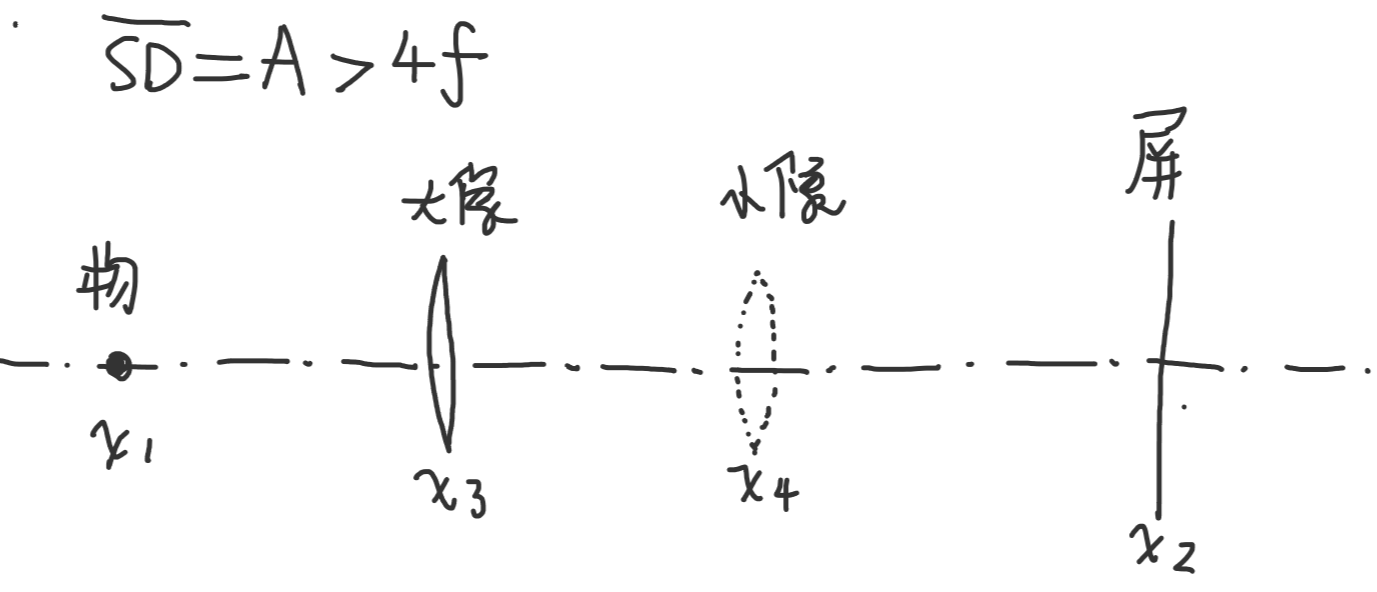
\includegraphics[scale=0.3]{weiyifa.png}
				\caption{位移法测量凸透镜焦距光路图}
			\end{figure}
			\par
			自准直法是将物置于透镜焦点的位置,物上每一点发出的光经过透镜折射变为平行光,再经过其后的平面镜
			反射,光线重新经过透镜,在原物中心对称的位置呈现出一个等大实像。
			\begin{figure}[h]
				\centering
				\label{自准直法光路图}
				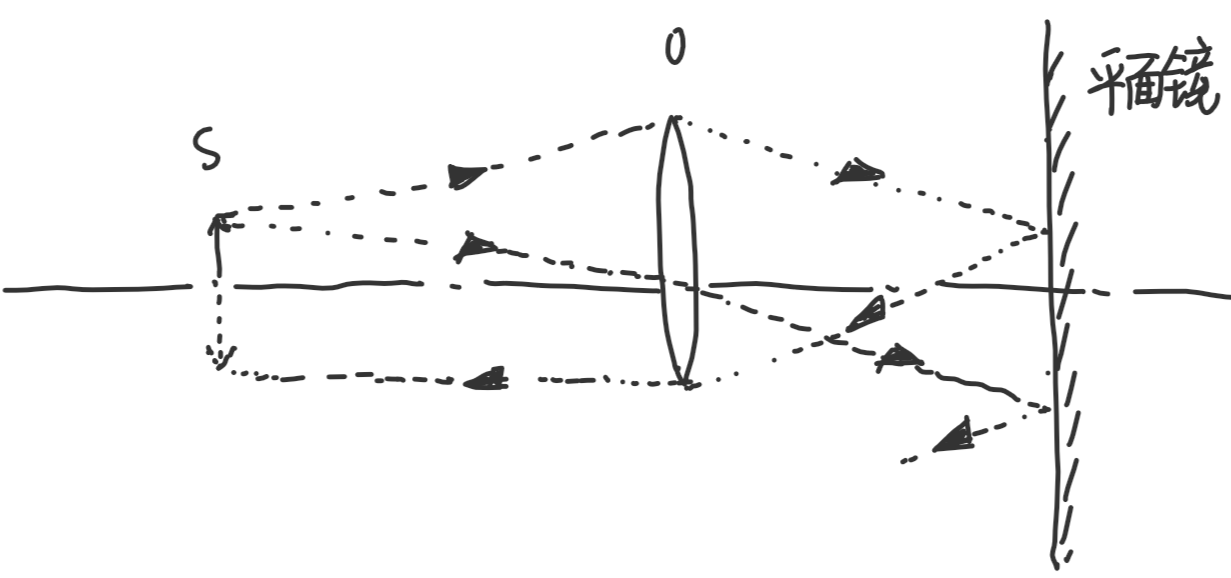
\includegraphics[scale=0.3]{zizhunzhifa.png}
				\caption{自准直法测量凸透镜焦距光路图}
			\end{figure}
			\par
			使用位移法测量时需要读取较多的数据,进行一定的计算,而且在实验操作上比较复杂,但是其可以选取
			不同的$A$值多次实验,因而可以比较准确地测量出凸透镜地焦距。使用自准直法测量时操作、计算都非常的简洁,但由于其无法改变参数多次实验(因为这样的操作意义并不大,如果实验中光路本身出了问题,那
			么无论如何在光学导轨上平移这些器件,都会得到相同的结果),这样的测量受偶然因素影响更大。
		\subsection{实验中测量误差的来源分析}
			\par 
			从实验条件的角度来看,长度的读数应该是一个会产生误差的地方,滑块上标示刻度的指针不与导轨上的刻
			度共面,所以读数时应该视线垂直于导轨读数,但是由于导轨较长,这样的操作比较麻烦,很有可能实验者
			为了方便而导致读数不准确,同时由于光学实验室内光线昏暗,所以也对读数造成了一定的困难。
			\par 
			在测量凸透镜的焦距时,明显可以看出数据的相对标准偏差很小,而对于凹透镜来说,焦距的相对标准偏差
			较大,这是和测量时的实验现象有关的。在对凸透镜进行测量时,光屏上物的实像的清晰程度对于距离很是
			敏感,很容易判断出在哪个距离下像最清晰,因此$l$的数值不确定度很小,自然会导致计算所得的$f$数
			值波动较小。在对凹透镜进行测量时,我们发现在相当距离范围内移动光屏,都会呈现出较为清晰的像。我
			们知道在固定了光屏与物之间的距离后,在其中间移动凸透镜会在光屏中呈现大像与小像两个大小不同的实
			像,观察表\ref{物像距法测量凹透镜焦距},其中第一个数据是利用凸透镜呈现的大像为凹透镜的虚像进
			行测量的,2、3是利用凹透镜呈现的小像进行测量的。利用大像作为虚像时,光屏中会呈现一个比实物大得多的暗淡的虚像,其清晰的边缘不便于确认;而利用小像作为虚像时,光屏中的像相对较小较明亮,边缘
			便于确认,所以这样测量更为准确一些,2、3组的结果更为接近也印证了这一点。但是值得注意的是,并不
			是小像越小越好,因为凸透镜距离实物越远所成的像越小,此时像距也会缩小(越来越接近焦距),如果
			向其中加入一面凹透镜,那么势必会导致物距的大小在10cm之下,减少了有效数字,会极大地提高误差。
\end{document}